%%%%%%%%%%%%%%%%%%%%%%%%%%%%%%%%%%%%%%%%%%%%%%%%%%%%%%%%%%%%%%%%%%%%%%%%%%%%%%%%
%
% Template license:
% CC BY-NC-SA 3.0 (http://creativecommons.org/licenses/by-nc-sa/3.0/)
%
%%%%%%%%%%%%%%%%%%%%%%%%%%%%%%%%%%%%%%%%%%%%%%%%%%%%%%%%%%%%%%%%%%%%%%%%%%%%%%%%

%----------------------------------------------------------------------------------------
%	PACKAGES AND OTHER DOCUMENT CONFIGURATIONS
%----------------------------------------------------------------------------------------

\documentclass[
11pt, % The default document font size, options: 10pt, 11pt, 12pt
%oneside, % Two side (alternating margins) for binding by default, uncomment to switch to one side
%chapterinoneline,% Have the chapter title next to the number in one single line
spanish,
singlespacing, % Single line spacing, alternatives: onehalfspacing or doublespacing
%draft, % Uncomment to enable draft mode (no pictures, no links, overfull hboxes indicated)
%nolistspacing, % If the document is onehalfspacing or doublespacing, uncomment this to set spacing in lists to single
%liststotoc, % Uncomment to add the list of figures/tables/etc to the table of contents
%toctotoc, % Uncomment to add the main table of contents to the table of contents
parskip, % Uncomment to add space between paragraphs
codirector, % Uncomment to add a codirector to the title page
headsepline, % Uncomment to get a line under the header
]{MastersDoctoralThesis} % The class file specifying the document structure



%----------------------------------------------------------------------------------------
%	INFORMACIÓN DE LA MEMORIA
%----------------------------------------------------------------------------------------

\thesistitle{Sistema de monitoreo y control de ambientes a distancia} % El títulos de la memoria, se usa en la carátula y se puede usar el cualquier lugar del documento con el comando \ttitle

% Nombre del posgrado, se usa en la carátula y se puede usar el cualquier lugar del documento con el comando \degreename
%\posgrado{Carrera de Especialización en Sistemas Embebidos} 
\posgrado{Carrera de Especialización en Internet de las Cosas} 
%\posgrado{Carrera de Especialización en Intelegencia Artificial}
%\posgrado{Maestría en Sistemas Embebidos} 
%\posgrado{Maestría en Internet de las cosas}

\author{César Javier Fanelli} % Tu nombre, se usa en la carátula y se puede usar el cualquier lugar del documento con el comando \authorname

\director{Ing. Fernando Lichtschein (FIUBA)} % El nombre del director, se usa en la carátula y se puede usar el cualquier lugar del documento con el comando \dirname
\codirector{Ing. María Celeste Corominas (FIUBA)} % El nombre del codirector si lo hubiera, se usa en la carátula y se puede usar el cualquier lugar del documento con el comando \codirname.  Para activar este campo se debe descomentar la opción "codirector" en el comando \documentclass, línea 23.

\juradoUNO{Esp. Ing. Pedro Rosito (FIUBA)} % Nombre y pertenencia del un jurado se usa en la carátula y se puede usar el cualquier lugar del documento con el comando \jur1name
\juradoDOS{Ing. Marcelo Edgardo Romeo (UNSAM)} % Nombre y pertenencia del un jurado se usa en la carátula y se puede usar el cualquier lugar del documento con el comando \jur2name
\juradoTRES{Nombre del jurado 3 (pertenencia)} % Nombre y pertenencia del un jurado se usa en la carátula y se puede usar el cualquier lugar del documento con el comando \jur3name

\ciudad{Ciudad Autónoma de Buenos Aires}
%\ciudad{ciudad de Mendoza}

\fechaINICIO{febrero de 2023}
\fechaFINAL{diciembre de 2023}


\keywords{Internet de las cosas, FIUBA} % Keywords for your thesis, print it elsewhere with \keywordnames


\begin{document}


\frontmatter % Use roman page numbering style (i, ii, iii, iv...) for the pre-content pages

\pagestyle{plain} % Default to the plain heading style until the thesis style is called for the body content


%----------------------------------------------------------------------------------------
%	RESUMEN - ABSTRACT 
%----------------------------------------------------------------------------------------

\begin{abstract}
\addchaptertocentry{\abstractname} % Add the abstract to the table of contents
%
%The Thesis Abstract is written here (and usually kept to just this page). The page is kept centered vertically so can expand into the blank space above the title too\ldots
\centering

%El resumen debe escribirse en uno o dos párrafo.  Debe ser breve y conciso sin ningún elemento de formato en el texto como itálicas o negrita. Tampoco se deben usar siglas ni acrónimos que no resulten obvios para un lector promedio de la memoria, ni referencias bibliográficas o notas al pie de página.  No debe faltar qué es lo que se hizo/logró, qué importancia/valor tiene el proyecto/resultado, qué va a encontrar el lector en la memoria y qué contenidos de la especialización/maestría se aplicaron en el proyecto.

En la presente memoria se describe el diseño de un prototipo de sistema integral de domótica de índole académica. El trabajo realizado abarca el diseño de una página web, el código de un servidor, código y hardware de los nodos, que permite controlar la intensidad de iluminación y la temperatura de la calefacción de las habitaciones de una casa.
El servidor se encuentra instalado de forma local y conectado a la red, montado sobre una Raspberry Pi, el cual aloja el frontend de la página web desde donde se pueden visualizar y cambiar los parámetros, el backend que recibe la información del frontend y la base de datos donde se alojan las mediciones, dispositivos y usuarios para iniciar sesión en el sistema. El otro componente del sistema es un nodo que recibe los parámetros enviados desde el servidor y cambia el estado de las salidas, y envía los parámetros sensados a la base de datos. En este caso se implementa un solo nodo, pero la idea es que sea escalable y se implementen los que sean necesarios. El nodo tiene también un selector de estado para cambiar las salidas y un display donde mostrará los parámetros sensados y seteados. Esto es para que funcione en modo independiente sin necesidad de comunicarse con el servidor o en caso de ser necesario cambiar los estados desde la habitación.

\end{abstract}

%----------------------------------------------------------------------------------------
%	CONTENIDO DE LA MEMORIA  - AGRADECIMIENTOS
%----------------------------------------------------------------------------------------

\begin{acknowledgements}
%\addchaptertocentry{\acknowledgementname} % Descomentando esta línea se puede agregar los agradecimientos al índice
\vspace{1.5cm}

%Esta sección es para agradecimientos personales y es totalmente \textbf{OPCIONAL}.  

Agradezco a docentes, alumnos y no docentes que conforman el posgrado y a los directores que me acompañaron en el desarrollo de este trabajo. En especial agradezco a mi esposa e hija, quienes fueron mi apoyo en todo momento y sin quienes no habría podido lograr la hazaña de emprender este viaje arduo y satisfactorio.

\end{acknowledgements}

%----------------------------------------------------------------------------------------
%	LISTA DE CONTENIDOS/FIGURAS/TABLAS
%----------------------------------------------------------------------------------------

\tableofcontents % Prints the main table of contents

\listoffigures % Prints the list of figures

\listoftables % Prints the list of tables


%----------------------------------------------------------------------------------------
%	CONTENIDO DE LA MEMORIA  - DEDICATORIA
%----------------------------------------------------------------------------------------

\dedicatory{\textbf{Dedicado a mi hija Sofía.}}  % escribir acá si se desea una dedicatoria

%----------------------------------------------------------------------------------------
%	CONTENIDO DE LA MEMORIA  - CAPÍTULOS
%----------------------------------------------------------------------------------------

\mainmatter % Begin numeric (1,2,3...) page numbering

\pagestyle{thesis} % Return the page headers back to the "thesis" style

% Incluir los capítulos como archivos separados desde la carpeta Chapters

% Chapter 1

\chapter{Introducción general} % Main chapter title

\label{Chapter1} % For referencing the chapter elsewhere, use \ref{Chapter1} 
\label{IntroGeneral}

%----------------------------------------------------------------------------------------

% Define some commands to keep the formatting separated from the content 
\newcommand{\keyword}[1]{\textbf{#1}}
\newcommand{\tabhead}[1]{\textbf{#1}}
\newcommand{\code}[1]{\texttt{#1}}
\newcommand{\file}[1]{\texttt{\bfseries#1}}
\newcommand{\option}[1]{\texttt{\itshape#1}}
\newcommand{\grados}{$^{\circ}$}

%----------------------------------------------------------------------------------------

%\section{Introducción}

%----------------------------------------------------------------------------------------
\section{Introducción a la domótica}

La domótica es la aplicación de la tecnología a la automatización del hogar y de edificios que utiliza para controlar y gestionar diferentes sistemas y dispositivos en el hogar o edificio de forma automatizada, con el fin de aportar seguridad, bienestar y confort. Estos sistemas pueden incluir iluminación, calefacción, aire acondicionado, sistemas de seguridad y cámaras de vigilancia, sistemas de entretenimiento y otros dispositivos domésticos. \citep{1}

Este sector como muchos otros que utilizan tecnología ha estado creciendo, al punto que algunas de las viviendas modernas son concebidas como hogares inteligentes desde su edificación, llegando a tener edificios completos con este tipo de soluciones instaladas.

\subsection{Aplicaciones}

Los servicios que ofrece la domótica se pueden agrupar según cinco aspectos o ámbitos principales\citep{2}:

\begin{itemize}
	\item Programación y ahorro energético. El ahorro energético no es algo tangible, sino legible con un concepto al que se puede llegar de muchas maneras. En muchos casos no es necesario sustituir los aparatos o sistemas del hogar por otros que consuman menos energía sino una gestión eficiente de los mismos.
	\item Confort. El confort conlleva todas las actuaciones que se puedan llevar a cabo que mejoren la comodidad en una vivienda. Dichas actuaciones pueden ser de carácter tanto pasivo, como activo o mixtas.
	\item Seguridad. Consiste en una red de seguridad encargada de proteger tanto los bienes patrimoniales, como la seguridad personal y la vida.
	\item Comunicaciones. Son los sistemas o infraestructuras de comunicaciones que posee el hogar.
	\item Accesibilidad. Bajo este mecanismo se incluyen las aplicaciones o instalaciones de control remoto del entorno que favorecen la autonomía personal de personas con limitaciones funcionales, o discapacidad.
\end{itemize}


\chapter{Introducción específica} % Main chapter title

\label{Chapter2}

En el presente capítulo se introducen las tecnologías y herramientas de hardware y software utilizados en el desarrollo del trabajo. 

\section{Protocolos de comunicación}
\subsection{Modelo OSI}

El modelo de interconexión de sistemas abiertos, conocido como modelo OSI (en inglés, \textit{Open Systems Interconnection}), es un modelo de referencia para los protocolos de la red. Define un estándar que tiene por objetivo interconectar sistemas de distinta procedencia para que estos puedan intercambiar información sin ningún tipo de impedimentos. Está conformado por 7 capas o niveles de abstracción. Cada uno de estos niveles tiene sus propias funciones para que en conjunto sean capaces de poder alcanzar su objetivo final. Precisamente esta separación en niveles hace posible la intercomunicación de protocolos distintos al concentrar funciones específicas en cada nivel de operación \citep{8}.

En la figura \ref{fig:5} pueden verse de forma gráfica las distintas capas del modelo OSI.

\begin{figure}[h]
\centering
\includegraphics[scale=0.43]{Figura 5 - Modelo OSI.jpg}
\caption[Modelo OSI]{Modelo OSI. \footnotemark}
\label{fig:5}
\end{figure}
\footnotetext{Imagen tomada de: \url{https://platzi.com/clases/2225-redes/35587-modelo-osi/}}

A continuación se presentan en detalle las funciones de cada capa:

\begin{itemize}
	\item Capa 1 o física: define todas las especificaciones eléctricas y físicas de los dispositivos.
	\item Capa 2 o de enlace de datos: proporciona direccionamiento físico y procedimientos de acceso a medios.
	\item Capa 3 o de red: se encarga del direccionamiento lógico y el dominio del enrutamiento.
	\item Capa 4 o de transporte: proporciona transporte confiable y control del flujo a través de la red.
	\item Capa 5 o de sesión: establece, administra y finaliza las conexiones entre las aplicaciones locales y las remotas.
	\item Capa 6 de presentación: transforma el formato de los datos y proporciona una interfaz estándar para la capa de aplicación.
	\item Capa 7 o de aplicación: responsable de los servicios de red para las aplicaciones.
\end{itemize}

\subsection{Protocolo HTTP}

El protocolo de transferencia de hipertexto, conocido como HTTP (en inglés \textit{Hypertext Transfer Protocol}), es el protocolo de comunicación que permite las transferencias de información a través de archivos como XML y HTML entre otros. Está orientado a transacciones y sigue el esquema petición y respuesta entre un cliente y un servidor. El cliente realiza una petición al servidor enviando un mensaje con un formato determinado. El servidor le envía un mensaje de respuesta con la información solicitada o un mensaje de error \citep{9}.

Los mensajes HTTP son en texto plano y tienen la siguiente estructura:

\begin{itemize}
	\item Línea inicial.
	\item Cabecera.
	\item Cuerpo.
\end{itemize}

En la línea inicial, se envían las peticiones con el método hacia el servidor o las respuestas con el código devueltas hacia el navegador. Los métodos más comunes, y utilizados en el proyecto, son:

\begin{itemize}
	\item GET: solicita una representación del recurso especificado.
	\item POST: envía datos para que sean procesados por el recurso identificado en la URL de la línea de petición.
	\item PUT: envía datos al servidor. La diferencia con POST es que este está orientado a la creación de nuevos contenidos, mientras que PUT está orientado a la actualización de los mismos.
	\item DELETE: Borra el recurso especificado.
\end{itemize}

\subsection{Protocolo MQTT}

El protocolo de transporte de telemetría de colas de mensajes, conocido como MQTT (en inglés \textit{Message Queue Telemetry Transport}) es uno de los más utilizados y difundidos en IoT (Internet de las cosas, o en inglés \textit{Internet of Things}). Es un protocolo de capa de aplicación, posee una topología de estrella, y sus mensajes se transmiten como colas de publicación/suscripción.

El nodo central de su topología se llama \textit{broker} y es al cual se conectan los clientes remotos. El \textit{broker} se encarga de gestionar la red, recibir todos los mensajes de los clientes y redirigirlos hacia los clientes de destino. Un cliente es cualquier dispositivo que pueda interactuar con el \textit{broker} para enviar y recibir mensajes. Puede ser un sensor de IoT en campo o una aplicación en un centro de datos que procesa datos provenientes de los sensores. Cualquier cliente puede publicar o suscribirse a \textit{topics} (temas) para acceder a la información. Un \textit{topic} se representa mediante una cadena de texto con una estructura jerárquica. Cada jerarquía se separa con el caracter "/".

La finalidad de MQTT es minimizar el uso recursos en los dispositivos (CPU, RAM, ROM), ser confiable y ofrecer distintos niveles calidad del servicio. Consume un ancho de banda relativamente bajo y mantiene una conexión continua entre el broker y los clientes. Generalmente se suele usar este protocolo como nexo entre los dispositivos de campo con elementos típicos de software como servidores webs, bases de datos o herramientas de análisis. En la figura \ref{fig:6} se puede ver una arquitectura básica de conexión MQTT \citep{10}.

\begin{figure}[h]
\centering
\includegraphics[scale=0.96]{Figura 6 - Arquitectura MQTT.png}
\caption[Arquitectura MQTT]{Arquitectura MQTT. \footnotemark}
\label{fig:6}
\end{figure}
\footnotetext{Imagen tomada de: \url{https://www.twilio.com/blog/what-is-mqtt}}

Para reforzar la seguridad en la comunicación mediante MQTT, se pueden proteger los datos mediante el uso de usuario y contraseña, o con cifrado de capa de sockets seguros, conocidos como SSL (en inglés \textit{Secure Sockets Layer}). La capa de transporte segura (en inglés \textit{Transport Layer Security} o TLS), es una versión actualizada y más segura de SSL, y es por esto que en la actualidad se refiere a SSL/TLS como sinónimos.

\subsubsection{Calidad de servicio}

MQTT está diseñado para ser simple y minimizar el ancho de banda, lo que lo convierte en una buena opción para muchos escenarios, aunque esta simplicidad hace que la interpretación de los mensajes dependa completamente del diseñador del sistema. Para mitigar este tipo de inconvenientes se soportan distintos niveles de calidad de servicio.

Estos niveles determinan cómo se entrega cada mensaje y es necesario especificar un QoS (siglas en inglés para \textit{quality of service}) para cada \textit{topic} MQTT. Es importante elegir el valor de QoS adecuado para cada mensaje que está determinado de la siguiente manera:

\begin{itemize}
	\item QoS 0 (a lo sumo una vez): los mensajes se mandan sin tener en cuenta si llegan o no. Puede haber pérdida de mensajes. No se hacen retransmisiones.
	\item QoS 1 (al menos una vez): se asegura que los mensajes lleguen pero se pueden producir duplicados. El receptor recibe el mensaje por lo menos una vez. Si el receptor no confirma la recepción del mensaje o se pierde en el camino se reenvía el mensaje hasta que recibe por lo menos una confirmación.
	\item QoS 2 (exactamente una vez): se asegura que el mensaje llegue exactamente una vez. Eso incrementa la sobrecarga en la comunicación pero es la mejor opción cuando la duplicación de un mensaje no es aceptable.
\end{itemize}

\subsubsection{Protocolos SSL y TLS}

SSL y TLS son protocolos criptográficos, que proporcionan comunicaciones seguras por una red. Se usa criptografía asimétrica para autentificar a la contraparte con quien se está comunicando y para intercambiar una llave simétrica, iniciando una sesión entre las partes intervinientes. Esta sesión es luego usada para cifrar el flujo de datos entre las partes. Esto permite la confidencialidad de la información transmitida y la autenticación de los mensajes. 

Antes de que un cliente y el servidor pueden empezar a intercambiar información protegida por TLS, deben intercambiar en forma segura o acordar una clave de cifrado y una clave para usar cuando se cifren los datos. Existen varios métodos utilizados para el intercambio y acuerdo de claves \citep{11}.

\section{Componentes de hardware}

\subsection{Raspberry Pi}

Las Raspberry Pi son computadoras de placa simple (en inglés \textit{Single Board Computer} o su sigla SBC). Actualmente en el mercado existen distintas marcas y variantes de este tipo de placas, siendo elegidas tanto como computadoras de escritorio como para algunas aplicaciones específicas. A continuación, se describen las principales características de la familia Raspberry Pi:

\begin{itemize}
	\item Posee distintos puertos, permitiendo conectarla a periféricos como pueden ser una pantalla, un medio de almacenamiento e incluso cualquier dispositivo que tenga interfaz USB.
	\item Contiene un procesador gráfico integrado, lo que permite la reproducción de vídeo, incluso en alta definición.
	\item Permite la conexión a la red a través del puerto de Ethernet y algunos modelos permiten conexión Wi-Fi y Bluetooth.
	\item Consta de una ranura microSD que permite instalar y ejecutar sistemas operativos a través de una tarjeta de memoria.
\end{itemize}

El diseño de la Raspberry Pi fue evolucionando con el correr del tiempo. En la actualidad se encuentran los modelos Raspberry Pi 4 y Raspberry Pi 400, siendo los más modernos y robustos lanzados por la marca. La familia de Raspberry Pi 4 cuenta con 4 modelos de placa con distinta capacidad de memoria RAM, yendo desde 1 GB hasta 8 GB. La Raspberry Pi 400 es una variante de la Raspberry Pi 4. Además, existen otros modelos más pequeños diseñados para otro tipo de aplicaciones.

En la figura \ref{fig:7} se pueden ver los modelos Raspberry Pi 4 y Raspberry Pi 400.

\begin{figure}[h]
\centering
\includegraphics[scale=0.23]{Figura 7 - Raspberry.jpg}
\caption[Raspberry Pi 4 y Raspberry Pi 400]{Raspberry Pi 4 y Raspberry Pi 400. \footnotemark}
\label{fig:7}
\end{figure}
\footnotetext{Imagen tomada de: \url{https://all3dp.com/2/raspberry-pi-400-vs-raspberry-pi-4-differences/}}

Algunas de las funciones y aplicaciones más comunes de este tipo de computadoras se describen a continuación:

\begin{itemize}
	\item Navegar en la red, utilizar aplicaciones de oficina para la edición de documentos y emplearla como si fuese una computadora de escritorio.
	\item Crear un centro multimedia y ver los archivos guardados en su memoria.
	\item Se puede utilizar como un servidor privado dentro de una red local.
	\item Conectar los puertos del microprocesador desde un conector de 40 pines a distintos circuitos y dispositivos.
\end{itemize}

\subsubsection{Especificaciones técnicas de la Raspberry Pi 400}

El sistema operativo del servidor está instalado y se ejecuta desde un disco de estado sólido por USB. Este tipo de discos tienen una mayor capacidad de escrituras y lecturas que una memoria microSD, lo que resulta favorable al momento de hacer modificaciones y pruebas de ejecución de software. En la versión final del sistema todo el software estará instalado en una tarjeta microSD para que todo el conjunto sea lo más pequeño posible.

En la tabla \ref{tab:Especificaciones Raspberry Pi 400} pueden verse las especificaciones técnicas de hardware más importantes del modelo Raspberry Pi 400.

\begin{table}[h]
\centering
\caption[Especificaciones de Raspberry Pi 400]{Especificaciones de Raspberry Pi 400.}
\begin{tabular}{l c}
\toprule
Procesador		&	Broadcom BCM2711 quad-core Cortex-A72 (ARM v8) \\
				&	64-bit SoC @ 1.8 GHz \\
\midrule
Memoria			&	4GB LPDDR4-3200 \\
\midrule
				&	2.4 GHz and 5.0 GHz 802.11b/g/n/ac wireless LAN \\
Conectividad		&	Bluetooth 5.0, BLE\\
				&   Gigabit Ethernet \\
\midrule
Alimentación		&	5 V DC vía USB-C\\
\bottomrule
\hline
\end{tabular}
\label{tab:Especificaciones Raspberry Pi 400}
\end{table}

\subsection{Sistema en chip}
\label{subsection:SistemaEnChip}

Un sistema en chip o SoC (del inglés \textit{System on a Chip}) es aquel dispositivo que posee integrados todos o gran parte de los módulos que componen un sistema informático o electrónico en un único circuito integrado o chip. El diseño de estos sistemas puede estar basado en circuitos de señal digital, señal analógica y a menudo módulos o sistemas de radiofrecuencia. Un ámbito común de aplicación de la tecnología SoC son los sistemas embebidos.

Un SoC estándar está constituido por \citep{12}:

\begin{itemize}
	\item Un microcontrolador con el núcleo de la CPU. Algunos son construidos con microprocesadores dotados de varios núcleos.
	\item Módulos de memoria ROM (memoria de sólo lectura), RAM (memoria de acceso aleatorio), EEPROM (memoria de sólo lectura programable y borrable electrónicamente) y Flash (memorias de acceso muy rápido).
	\item Generadores de frecuencia fija.
	\item Componentes periféricos como contadores, temporizadores y relojes en tiempo real o RTC (en inglés \textit{Real Time Clock}).
	\item Controladores de comunicación con interfaces externas normalmente estándar como USB, Ethernet, UART, o SPI.
	\item Controladores de interfaces analógicas, incluyendo conversores analógico a digital (ADC) y digital a analógico (DAC).
	\item Reguladores de tensión y circuitos de gestión eficaz de la energía.
\end{itemize}

\subsubsection{Familia ESP32 \citep{13}}

ESP32 es la denominación de una familia de chips SoC de bajo costo y consumo de energía, con tecnología Wi-Fi y Bluetooth de modo dual integrada. Emplea un microprocesador Tensilica Xtensa LX6 en sus variantes de simple y doble núcleo e incluye interruptores de antena, balun de radiofrecuencia, amplificador de potencia, amplificador receptor de bajo ruido, filtros y módulos de administración de energía. El ESP32 fue creado y desarrollado por Espressif Systems.

En la figura \ref{fig:8} se pueden ver algunos de los módulos de desarrollo que contienen ESP32.

\begin{figure}[h]
\centering
\includegraphics[scale=0.6]{Figura 8 - Familia ESP32.jpg}
\caption[Módulos de la familia ESP32]{Módulos de la familia ESP32. \footnotemark}
\label{fig:8}
\end{figure}
\footnotetext{Imagen tomada de: \url{https://www.electrodaddy.com/esp32/}}

En la tabla \ref{tab:esp32} pueden verse las características de hardware más importantes del microcontrolador ESP32, utilizado para el desarrollo de los dispositivos.

\begin{table}[h]
\centering
\caption[Especificaciones técnicas del módulo ESP32]{Especificaciones técnicas del módulo ESP32 \citep{14}.}
\begin{tabular}{l c c}
\toprule
\textbf{Característica} & \textbf{ESP32}\\
\midrule
Núcleo			& Xtensa® dual-core 32-bit LX6\\
				& @240 MHz\\
Flash			& 0 MB, 2 MB o 4 MB\\
				& (dependiendo la versión)\\
Protocolo Wi-Fi	& 802.11 b/g/n, 2.4 GHz\\
\bottomrule
\hline
\end{tabular}
\label{tab:esp32}
\end{table}

\subsection{Especificaciones de los sensores}

A continuación, se listan sensores utilizados con sus principales características:

\begin{itemize}
	\item DHT22: sensor de temperatura y humedad relativa ambiente \citep{15}.
	\begin{itemize}
		\item Rango de temperatura: -40 a 80 grados Celsius.
		\item Resolución: 0,1 grado Celsius.
		\item Comunicación: serie, bus de 1 hilo, 40 bits por trama.
	\end{itemize}
	\item KY-040: encoder rotativo con interruptor. 20 pulsos por vuelta \citep{16}.
\end{itemize}

En la figura \ref{fig:9} se muestra la imagen del encoder a la izquierda y del sensor de temperatura a la derecha con sus correspondientes esquemas de conexión.

\newpage
\begin{figure}[h]
\centering
\includegraphics[scale=1.4]{Figura 9 - Sensores.jpg}
\caption[Sensores utilizados]{Sensores utilizados.}
\label{fig:9}
\end{figure}

\subsection{Especificaciones de los actuadores}

\begin{itemize}
\item SSD1306: display OLED 1,2 pulgadas \citep{17}.
	\begin{itemize}
		\item Resolución: 128x64 píxeles.
		\item Interfaz: I2C.
	\end{itemize}
	\item Control de potencia para 220 V: módulo con aislación y salida de triac. Se utilizó un triac BT137 \citep{18} y un optoacoplador MOC3041 \citep{19}.
	\begin{itemize}
		\item Tipo: encendido - apagado (on - off).
		\item Carga máxima: 8 A.
		\item Tipo de aislación: optoacoplador.
		\item Tensión máxima de aislación: 7500 V AC pico, 1 segundo de duración.
	\end{itemize}
	\item Control de intensidad de luz: módulo de control para iluminación LED de corriente continua implementado con modulación por ancho de pulso (PWM). Se utilizó un transistor BC337 \citep{20}.
	\begin{itemize}
		\item Tipo: PWM y encendido - apagado (on - off).
		\item Carga máxima: 800 mA CC.
		\item Tensión de alimentación: 5 a 24 V CC.
	\end{itemize}
\end{itemize}

En la figura \ref{fig:10} se muestra la imagen del circuito de potencia para la calefacción montado en una caja estanca a la izquierda, y del control por ancho de pulso para la dimerización a la derecha con sus correspondientes esquemas de conexión. Ambos circuitos fueron montados sobre una placa perforada de desarrollo para hacer las pruebas de funcionamiento.

\newpage
\begin{figure}[h]
\centering
\includegraphics[scale=1.3]{Figura 10 - Actuadores.jpg}
\caption[Actuadores utilizados]{Actuadores utilizados.}
\label{fig:10}
\end{figure}

\section{Herramientas de software}

\subsection{Visual studio code \citep{21}}

Visual Studio Code es un editor de código fuente desarrollado por Microsoft para múltiples sistemas operativos. Incluye soporte para la depuración, control integrado de Git, resaltado de sintaxis, finalización inteligente de código, fragmentos y refactorización de código. Es personalizable y tiene la posibilidad de instalar extensiones para agregar lenguajes, depuradores y herramientas para el desarrollo de código. Es gratuito y de código abierto, aunque la descarga oficial está bajo software privativo e incluye características personalizadas por Microsoft.

Algunos de los lenguajes de programación que soporta son: C, C++, Dockerfile, Git-commit, HTML, JSON, Java, JavaScript, PHP, Python, Ruby, Rust, SQL, Shell script, TypeScript y Visual Basic entre otros.

\subsection{Marco de desarrollo ESP}

El marco de desarrollo de ESP, o ESP-IDF (en inglés \textit{ESP IoT Development Framework}) es un entorno completo de programación para desarrollar sistemas embebidos para dispositivos ESP. Es desarrollado por Espressif y se puede descargar como una extensión de Visual studio code. El lenguaje de programación es C e incluye herramientas para cargar el código desarrollado al chip y depurar el programa en tiempo real.

El lenguaje C es un lenguaje de programación de propósito general de tipos de datos estáticos, débilmente tipado. Dispone de las estructuras típicas de los lenguajes de alto nivel pero, a su vez, dispone de construcciones del lenguaje que permiten un control a bajo nivel. Uno de los objetivos de diseño del lenguaje C es que solo sean necesarias unas pocas instrucciones en lenguaje máquina para traducir cada elemento del lenguaje, sin que haga falta un soporte intenso en tiempo de ejecución \citep{22}.

\subsection{Lenguajes JavaScript y TypeScript}

JavaScript (abreviado comúnmente JS) es un lenguaje de programación interpretado. Se define como orientado a objetos, basado en prototipos, imperativo, débilmente tipado y dinámico. Se utiliza principalmente del lado del cliente, implementado como parte de un navegador web permitiendo mejoras en la interfaz de usuario y páginas web dinámicas, aunque también se utiliza del lado del servidor. Todos los navegadores modernos interpretan el código en este lenguaje integrado en las páginas web. Para interactuar con una página web se provee al lenguaje JavaScript de una implementación del modelo de objeto de documento, o DOM (en inglés \textit{Document Object Model}). Es el único lenguaje de programación que entienden de forma nativa los navegadores \citep{23}.

TypeScript es un lenguaje de programación libre y de código abierto desarrollado y mantenido por Microsoft. Es un superconjunto de JavaScript, su antecesor, que esencialmente añade tipos estáticos y objetos basados en clases. Es usado para desarrollar aplicaciones JavaScript que se ejecutarán en el lado del cliente o del servidor, o extensiones para programas. Extiende la sintaxis de su antecesor, por tanto cualquier código en el lenguaje original existente debería funcionar sin problemas. Está pensado para grandes proyectos, los cuales a través de un compilador de TypeScript se traducen a código JavaScript \citep{24}.

\subsection{Angular y Ionic}

Angular es un marco de desarrollo (framework en inglés) de ingeniería de software de código abierto mantenido por Google, que sirve para desarrollar aplicaciones web de estilo aplicación de una sola página (en inglés \textit{single page application} o SPA) y aplicación web progresiva (en inglés \textit{Progressive Web App} o PWA). Sirve tanto para versiones móviles como de escritorio. Ofrece soluciones robustas, escalables y optimizadas para lograr un estilo de codificación homogéneo y de gran modularidad. Su desarrollo se realiza por medio de TypeScript o JavaScript. En este último se ofrecen diversas herramientas adicionales al lenguaje como tipado estático o decoradores \citep{25}.

El marco de desarrollo Ionic es un kit de desarrollo de software (en inglés \textit{Software Development Kit} o SDK) de frontend de código abierto para desarrollar aplicaciones híbridas basado en tecnologías web (HTML, CSS y JS). Es decir, un framework que nos permite desarrollar aplicaciones multiplataforma desde una única base de código. Posee la capacidad de integrarse con otros marcos populares como Angular, React y Vue. Su principal característica es que permite desarrollar y desplegar aplicaciones híbridas, que funcionan en múltiples plataformas, como iOS nativo, Android, escritorio y la web (como una aplicación web progresiva) con una única base de código \citep{26}.

\subsection{Bases de datos relacionales MySQL y MariaDB}

Una base de datos relacional es un conjunto de una o más tablas estructuradas en registros (filas) y campos (columnas), que se vinculan entre sí por un campo en común. MySQL es un sistema de administración de bases de datos relacionales de código abierto desarrollado por Oracle. Se considera como la base de datos de código abierto más utilizada en el mundo. Posee cuatro funciones básicas que se conocen con la sigla CRUD: \textit{create} (crear), \textit{read} (leer), \textit{update} (actualizar) y \textit{delete} (borrar). Estas funciones son las que se aplican a los nuevos registros que se quieran crear y a los ya existentes que se deseen leer, actualizar y borrar. Este tipo de bases de datos posee una arquitectura cliente-servidor, siendo el cliente el que hace las solicitudes de datos y el servidor el que posee dichos datos y responde a dicha solicitud.

MariaDB es una versión modificada de MySQL. Fue creada por el equipo de desarrollo original de MySQL debido a problemas de licencia y distribución después de que Oracle Corporation adquiriera MySQL. MariaDB adopta los archivos de definición de tablas y datos de MySQL y también usa protocolos de cliente, API de cliente, puertos y sockets idénticos. Con ello se pretende que los usuarios de MySQL puedan cambiar a MariaDB sin problemas \citep{27}.

\subsection{Contenedores con Docker}

Los contenedores son una forma de virtualización del sistema operativo. Un solo contenedor se puede usar para ejecutar cualquier aplicación, desde un microservicio o un proceso de software a una aplicación de mayor tamaño. Dentro de un contenedor se encuentran todos los ejecutables, el código binario, las bibliotecas y los archivos de configuración necesarios. Sin embargo, en comparación con los métodos de virtualización de máquinas o servidores, los contenedores no contienen imágenes del sistema operativo. Esto los hace más ligeros y portátiles, con una sobrecarga significativamente menor. En implementaciones de aplicaciones de mayor tamaño, se pueden poner en marcha varios contenedores como uno o varios clústeres de contenedores. Estos clústeres se pueden gestionar mediante un orquestador de contenedores, como Kubernetes o Docker Compose \citep{28}.

Docker es un proyecto de código abierto que automatiza el despliegue de aplicaciones dentro de contenedores de software, proporcionando una capa adicional de abstracción y automatización de virtualización de aplicaciones en múltiples sistemas operativos. Usar Docker para crear y gestionar contenedores puede simplificar la creación de sistemas altamente distribuidos, permitiendo que múltiples aplicaciones, las tareas de los trabajadores y otros procesos funcionen de forma autónoma en una única máquina física o en varias máquinas virtuales \citep{29}. En la figura \ref{fig:11} se puede ver de forma gráfica el funcionamiento de un contenedor Docker.

\begin{figure}[h]
\centering
\includegraphics[scale=0.4]{Figura 11 - Docker.jpg}
\caption[Contenedor Docker]{Contenedor Docker. \footnotemark}
\label{fig:11}
\end{figure}
\footnotetext{Imagen tomada de: \url{https://algodaily.com/lessons/what-is-a-container-a-docker-tutorial}}

Docker Compose es una herramienta para definir y ejecutar aplicaciones Docker de varios contenedores. Se utiliza un archivo YAML para configurar los servicios de su aplicación, y luego, con un solo comando, se crean e inician todos los servicios desde su configuración. Tiene comandos para gestionar todo el ciclo de vida de una aplicación con los que se pueden \citep{30}:

\begin{itemize}
	\item Iniciar, detener y reconstruir servicios.
	\item Ver el estado de los servicios en ejecución.
	\item Transmitir la salida del registro de los servicios en ejecución.
	\item Ejecutar un comando único en un servicio.
\end{itemize}
 
\chapter{Diseño e implementación}

\label{Chapter3}

En el presente capítulo se presentan los detalles del diseño y los criterios adoptados para el desarrollo del trabajo junto con los pasos seguidos para la implementación del mismo.

\section{Arquitectura del sistema}

La arquitectura del sistema es de cliente-servidor. Está constituido por dos nodos y un servidor, los cuales están conectados a la red local y se comunican a través del protocolo MQTT. De esta forma el servidor recibe los parámetros actuales de estado y cambios desde cada dispositivo, los procesa y almacena en la base de datos. También envía mensajes hacia los dispositivos para cambiar el estado de las salidas o el parámetro que se desee cambiar. Los usuarios pueden consultar y modificar el estado de los dispositivos desde un navegador web móvil o desde una computadora.

En la imagen \ref{fig:9} se puede observar una arquitectura típica cliente-servidor implementada con una Raspberry Pi.

\begin{figure}[h]
\centering
\includegraphics[scale=1.4]{Imagen 9 - cliente-servidor.jpg}
\caption[Arquitectura cliente-servidor]{Arquitectura cliente-servidor. \footnotemark}
\label{fig:9}
\end{figure}
\footnotetext{Imagen tomada de: \url{https://www.bujarra.com/raspberry-pi-servidor-vpn-con-pptp/}}

Uno de los nodos tiene como función sensar y controlar de temperatura de un recinto, y el otro controlar la iluminación. Originalmente el proyecto estaba pensado para que un solo nodo implemente estas dos funciones, pero durante el desarrollo se optó por la implementación separada. Este cambio se basó en la idea de modularizar los nodos y que sus funciones sean específicas. De esta forma es más amigable para el usuario visualizar y modificar el estado en pantalla e implementar el alta de nuevos dispositivos en el sistema.

El servidor está montado sobre una Raspberry Pi 400 con un sistema operativo Raspbian con interfaz gráfica. Este sistema operativo es la versión oficial ofrecida por la fundación Rasperry Pi y está basado en Debian versión 11 (\textit{bullseye}). En esta etapa de desarrollo se optó por una Raspberry Pi 400 por una cuestión de costos y practicidad a la hora de desarrollar y hacer las pruebas, aunque tiene un mayor volumen que los otros modelos de la familia. Al momento de ofrecer una solución definitiva está pensado que sea implementado en una placa con el formato más pequeño como cualquiera de las Raspberry Pi 4. La conexión del servidor a la red local es por cable ethernet.

\subsection{Especificaciones técnicas del servidor}

El sistema operativo del servidor está instalado y se ejecuta desde un disco de estado sólido por USB, que tiene una mayor capacidad de escrituras y lecturas que una memoria microSD. Esto favorece al momento de hacer pruebas en un desarrollo de este estilo.  El sistema operativo y todo el software adicional tendría que estar montado en una tarjeta SD para que todo el conjunto sea lo más pequeño posible.

En la tabla \ref{tab:Especificaciones Raspberry Pi 400} pueden verse las especificaciones técnicas de hardware más importantes del modelo Raspberry Pi 400.

\begin{table}[h]
\centering
\caption[Raspberry Pi 400]{Especificaciones de Raspberry Pi 400.}
\begin{tabular}{l c}
\toprule
Procesador		&	Broadcom BCM2711 quad-core Cortex-A72(ARM v8) \\
				&	64-bit SoC @ 1.8GHz \\
\midrule
Memoria			&	4GB LPDDR4-3200 \\
\midrule
				&	2.4GHz and 5.0GHz 802.11b/g/n/ac wireless LAN \\
Conectividad		&	Bluetooth 5.0, BLE\\
				&   Gigabit Ethernet \\
\midrule
Alimentación		&	5V DC vía USB-C\\
\bottomrule
\hline
\end{tabular}
\label{tab:Especificaciones Raspberry Pi 400}
\end{table}

\section{Modelo de datos}



\section{Desarrollo del frontend}



\section{Desarrollo del backend}



\section{Nodos, sensores y actuadores}



\section{Comunicación del sistema}
\chapter{Ensayos y resultados}

\label{Chapter4}

En este capítulo se detallan los ensayos realizados al sistema completo y los resultados obtenidos durante las pruebas de funcionamiento.

\section{Banco de pruebas}

El sistema consta físicamente de dos tipos de componentes: nodos y servidor. El servidor incluye tanto la aplicación en el frontend y el backend con sus respectivos módulos. Además, el sistema posee dos tipos de nodos: uno para el control de calefacción y otro para el control de iluminación.

Para ensayar el nodo de temperatura, se utilizaron los materiales que lo conforman que se muestran en la figura \ref{fig:31}.

\begin{figure}[h]
\centering
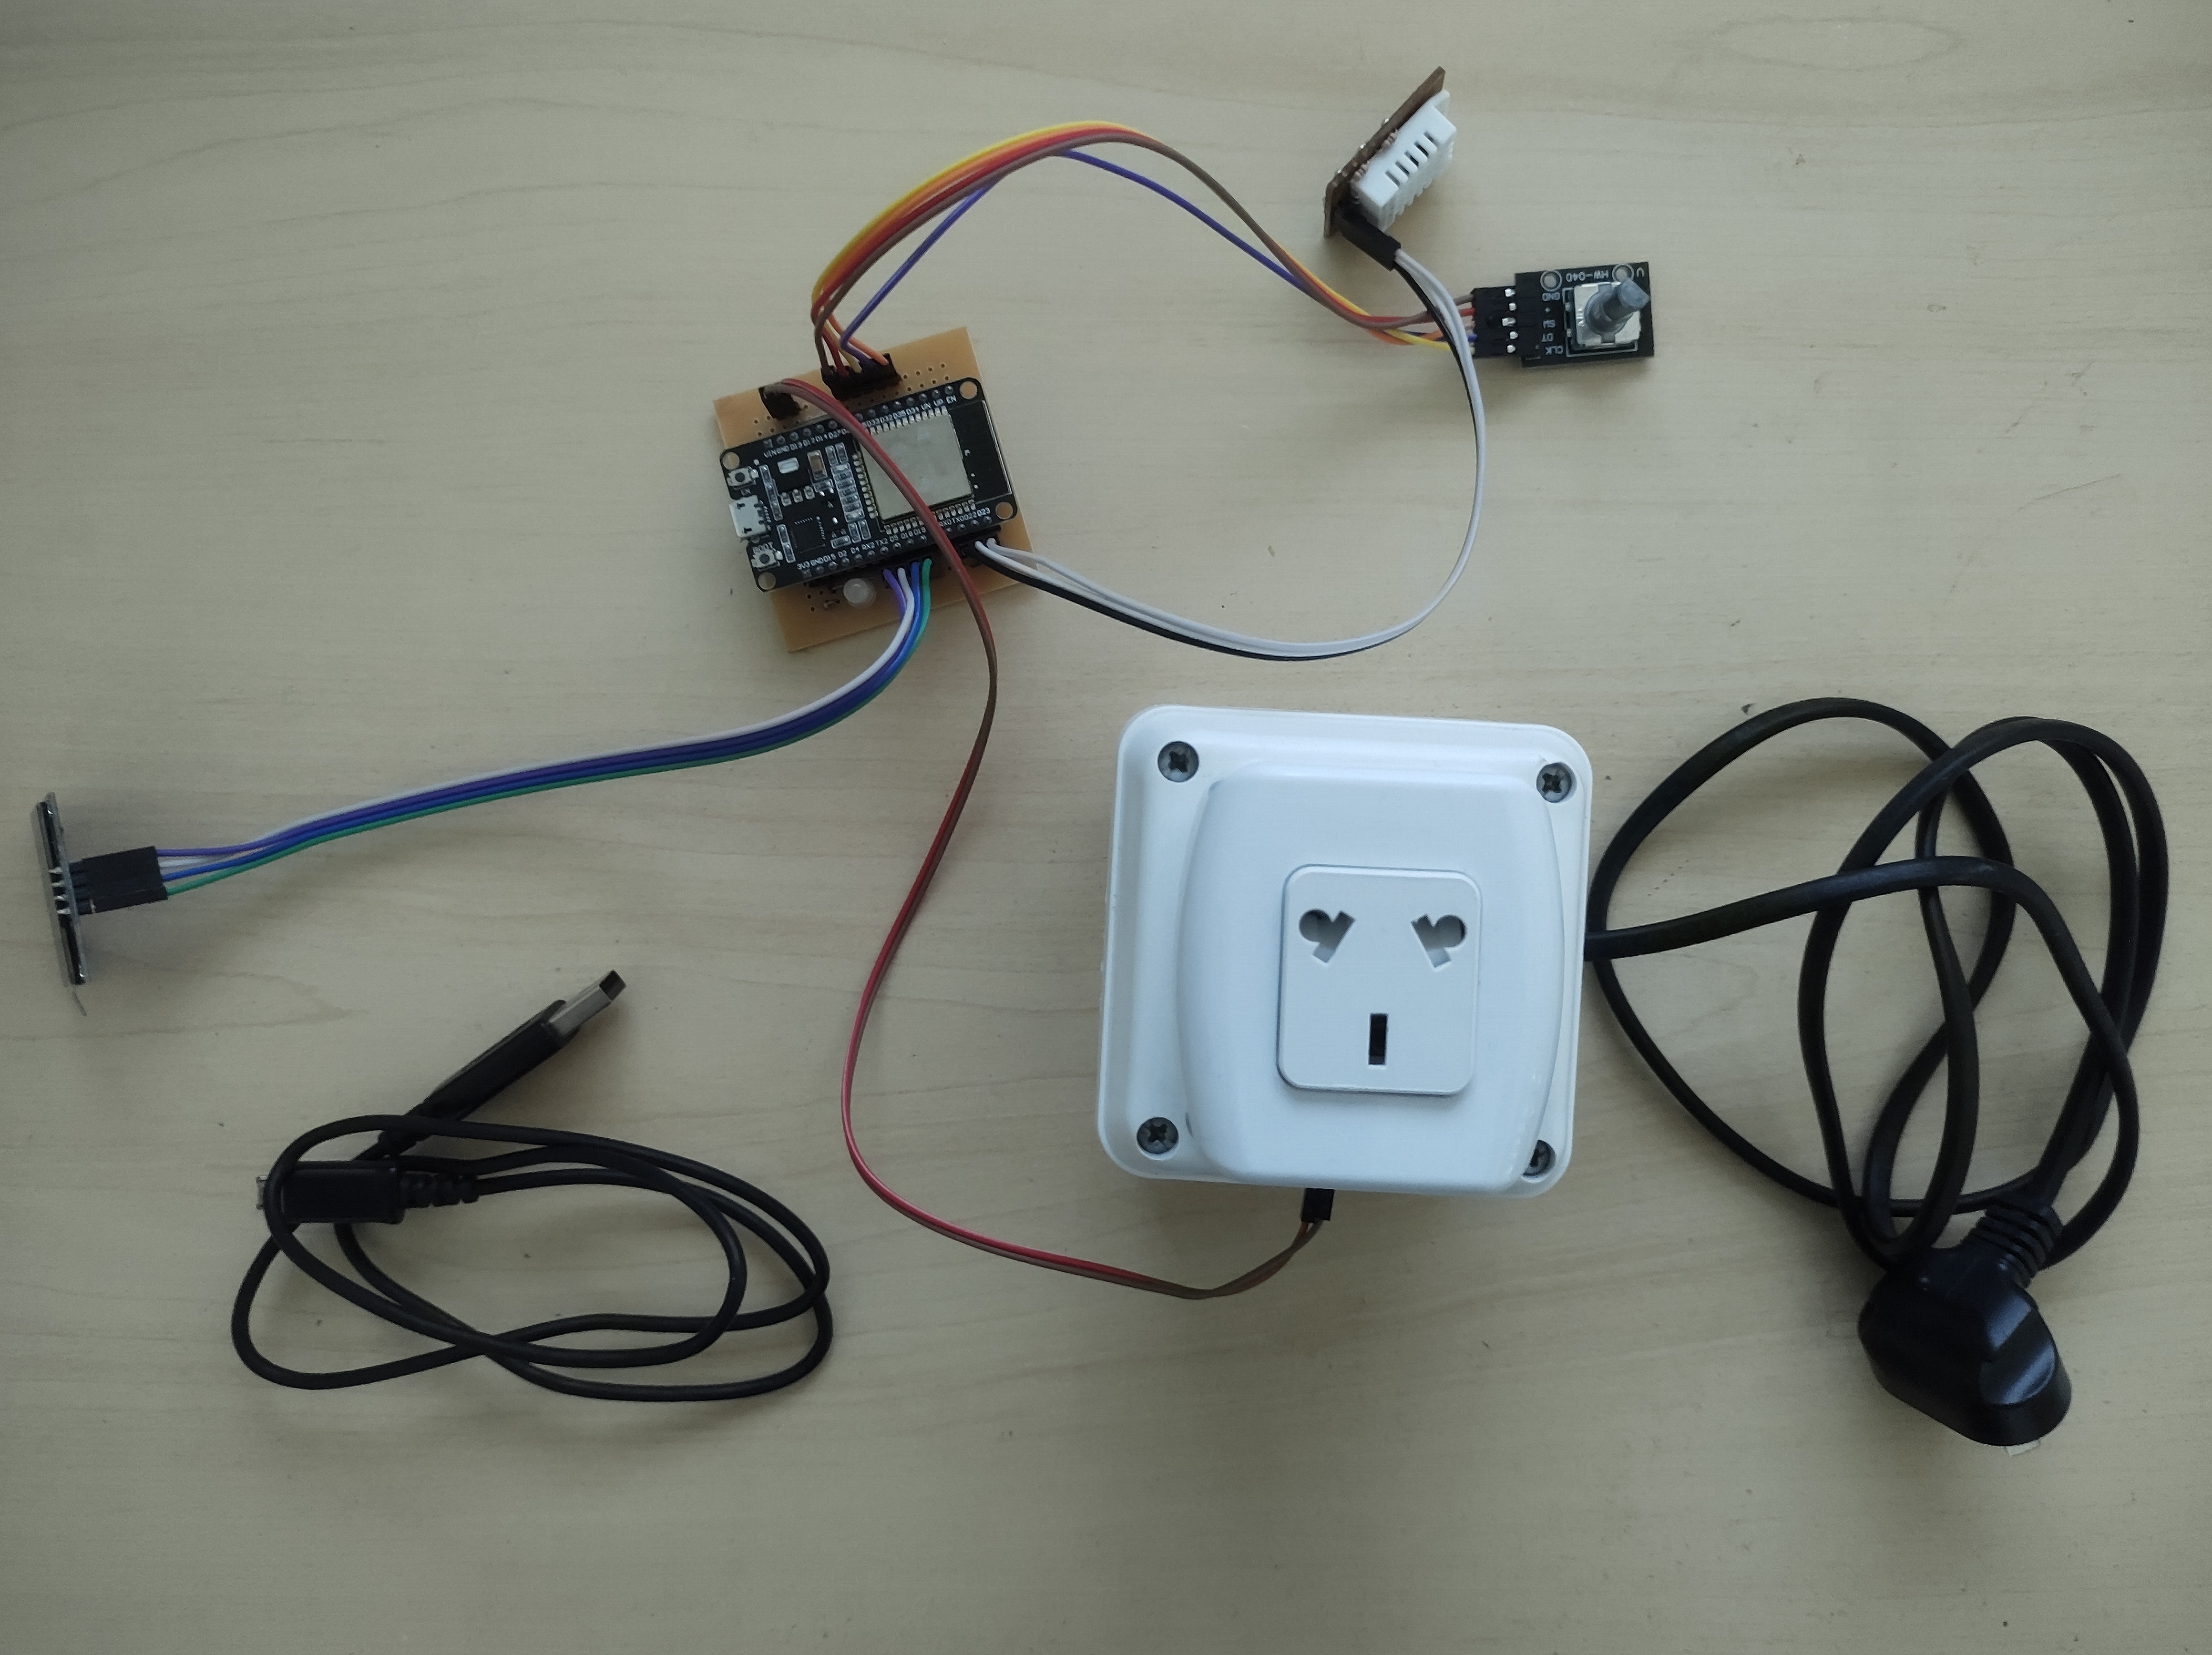
\includegraphics[scale=0.25]{Figura 31 - Nodo temperatura.jpg}
\caption[Componentes del nodo de temperatura]{Componentes del nodo de temperatura.}
\label{fig:31}
\end{figure}

En la figura \ref{fig:31}, se puede observar la placa ESP32 montada sobre la placa de conexiones, el display, el encoder, el sensor de temperatura y una caja estanca con una conexión de toma corriente para conectar la estufa a encender. Además, esta caja incluye un cable para conectarse a una fuente de alimentación de 220 VCA, que actúa como un interruptor. Cabe aclarar que en modo automático, el control de temperatura opera con una histéresis de 1 grado. Esto significa que al configurar una temperatura específica, el control apagará la salida cuando la temperatura supere en 1 grado al set-point y la encenderá cuando esté 1 grado por debajo de este valor.

Para ensayar el nodo de dimerización, se utilizaron los materiales que lo conforman que se muestran en la figura \ref{fig:32}.

\begin{figure}[h]
\centering
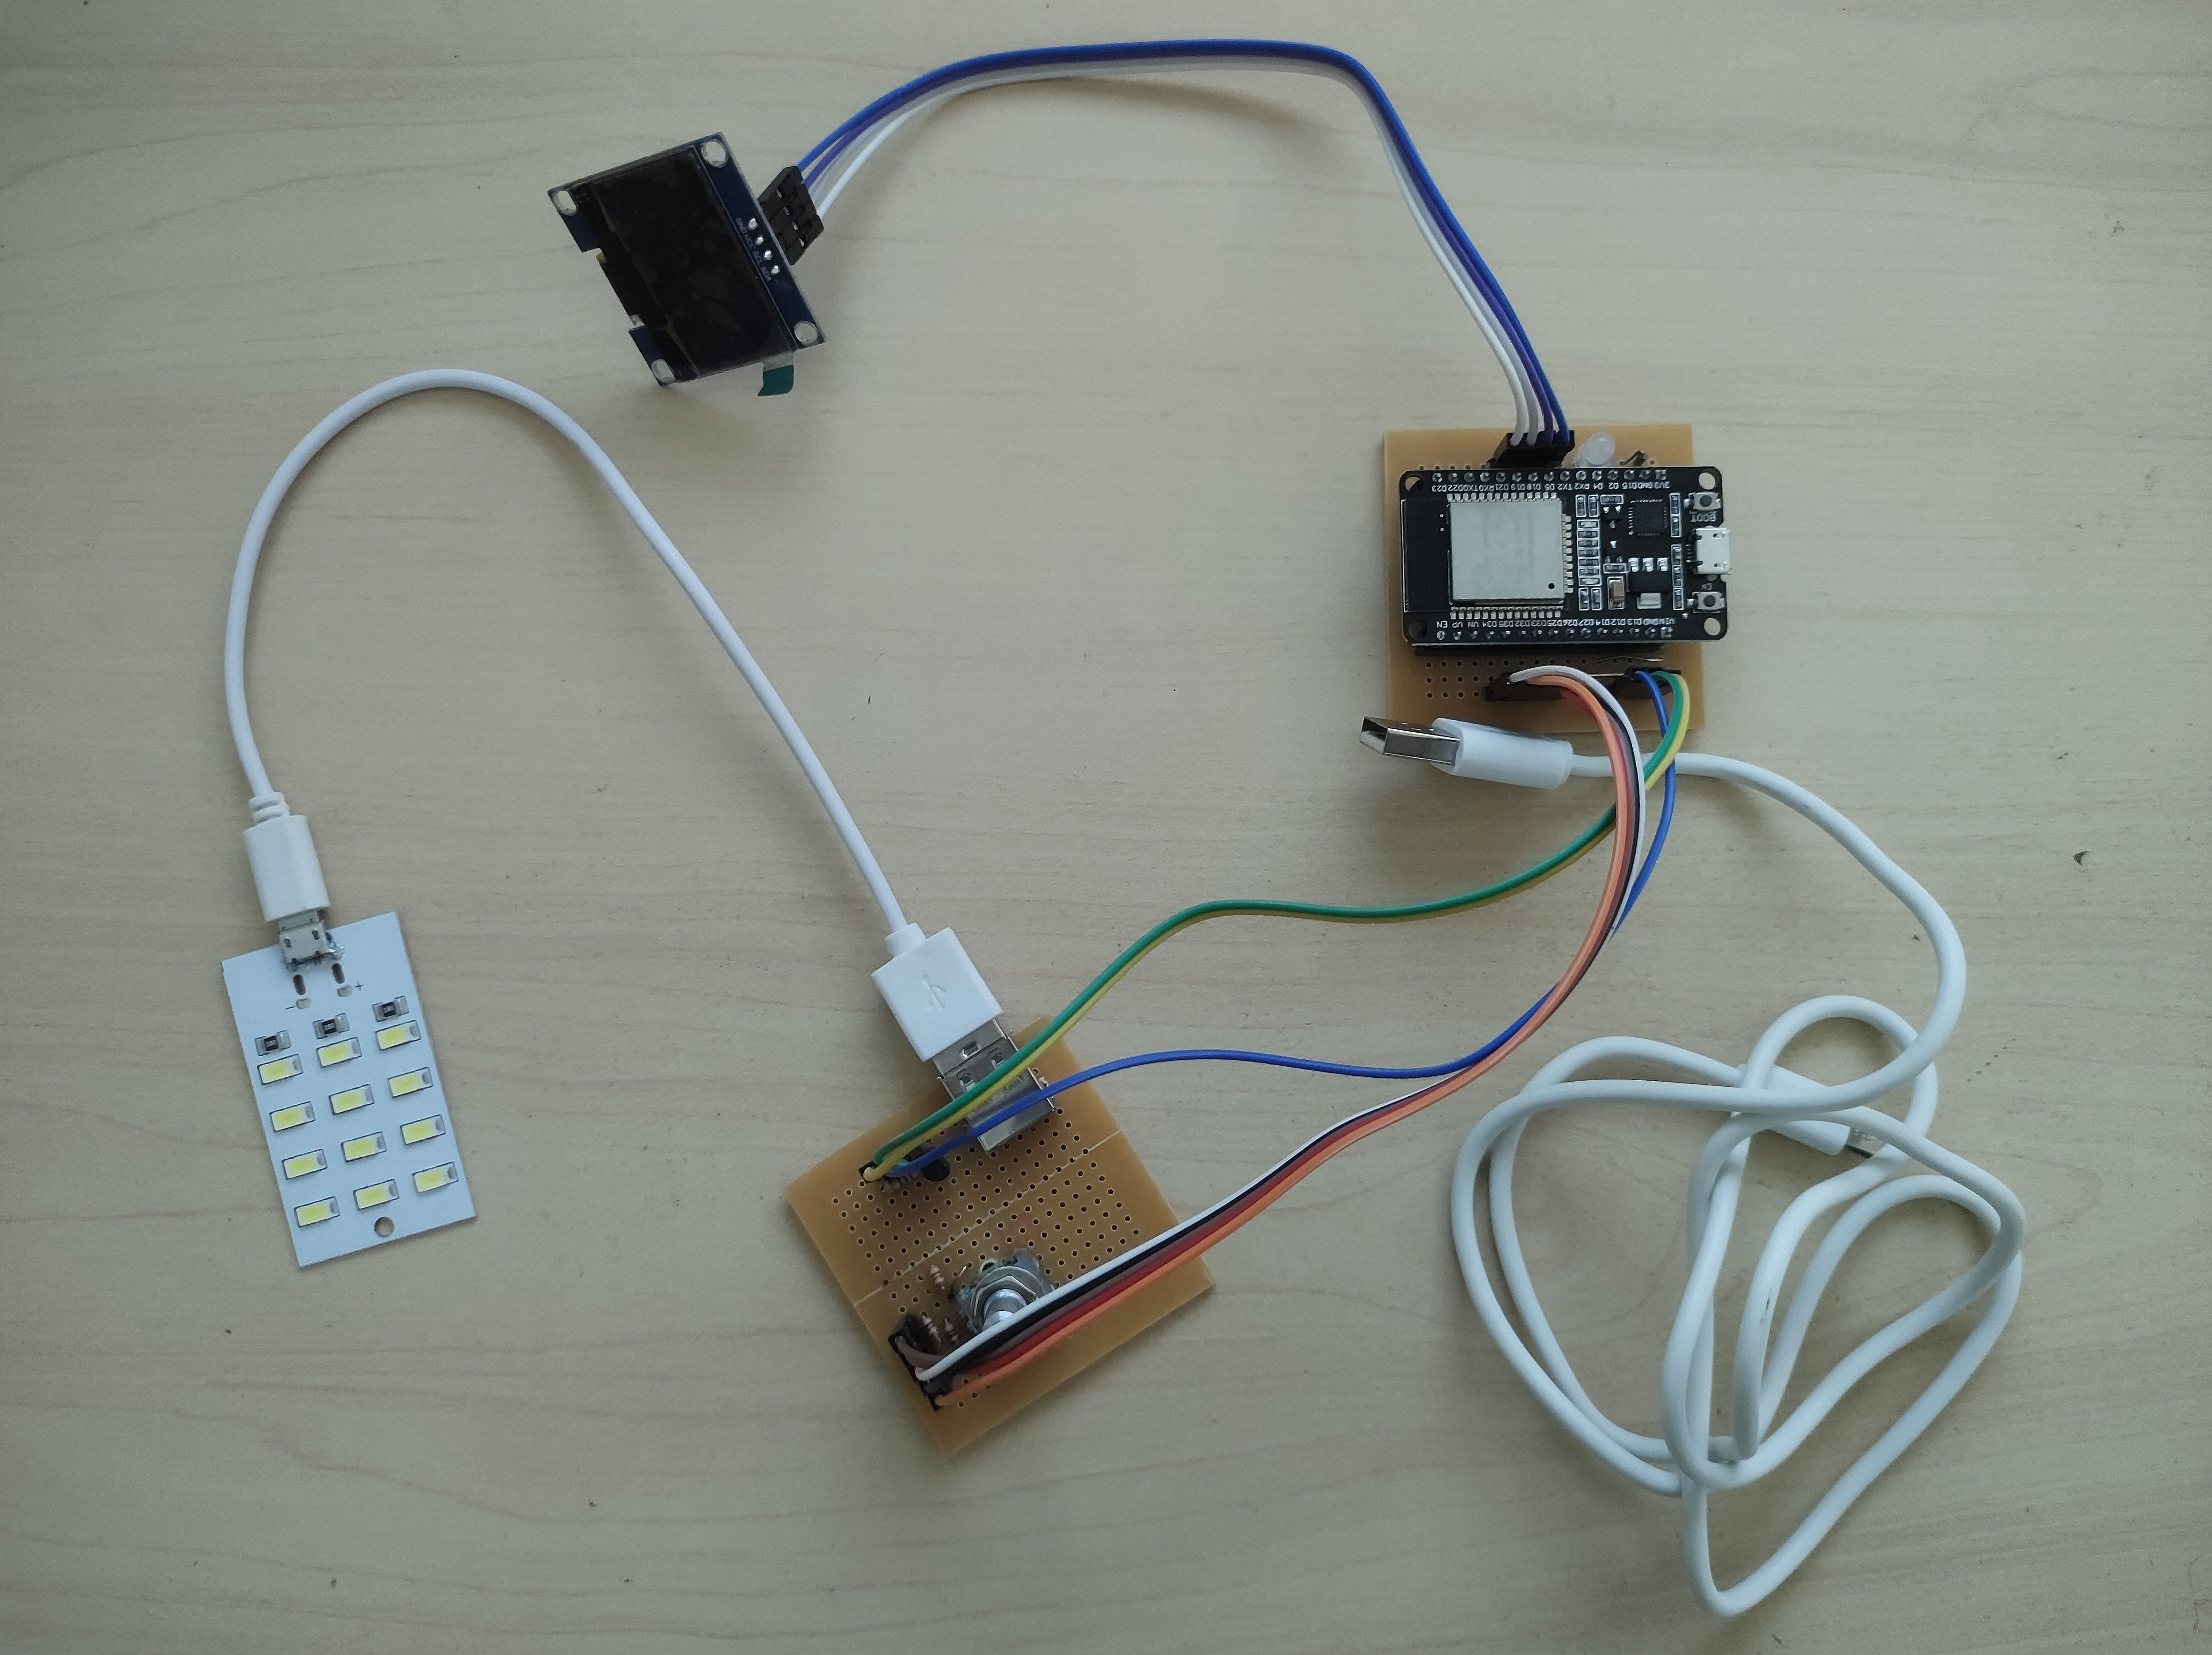
\includegraphics[scale=0.25]{Figura 32 - Nodo dimmer.jpg}
\caption[Componentes del nodo de dimerización]{Componentes del nodo de dimerización.}
\label{fig:32}
\end{figure}

En la figura  \ref{fig:32} se puede observar la placa ESP32 montada sobre la placa de conexiones, el display, el encoder, el \textit{driver} de iluminación y la placa de LEDs de 5 VCC. El control posee un conector USB por lo que puede conectarse cualquier lámpara que funcione en este caso con 5 VCC y posea este conector.

En la figura \ref{fig:33} pueden verse los componentes que forman parte del servidor.

\begin{figure}[h]
\centering
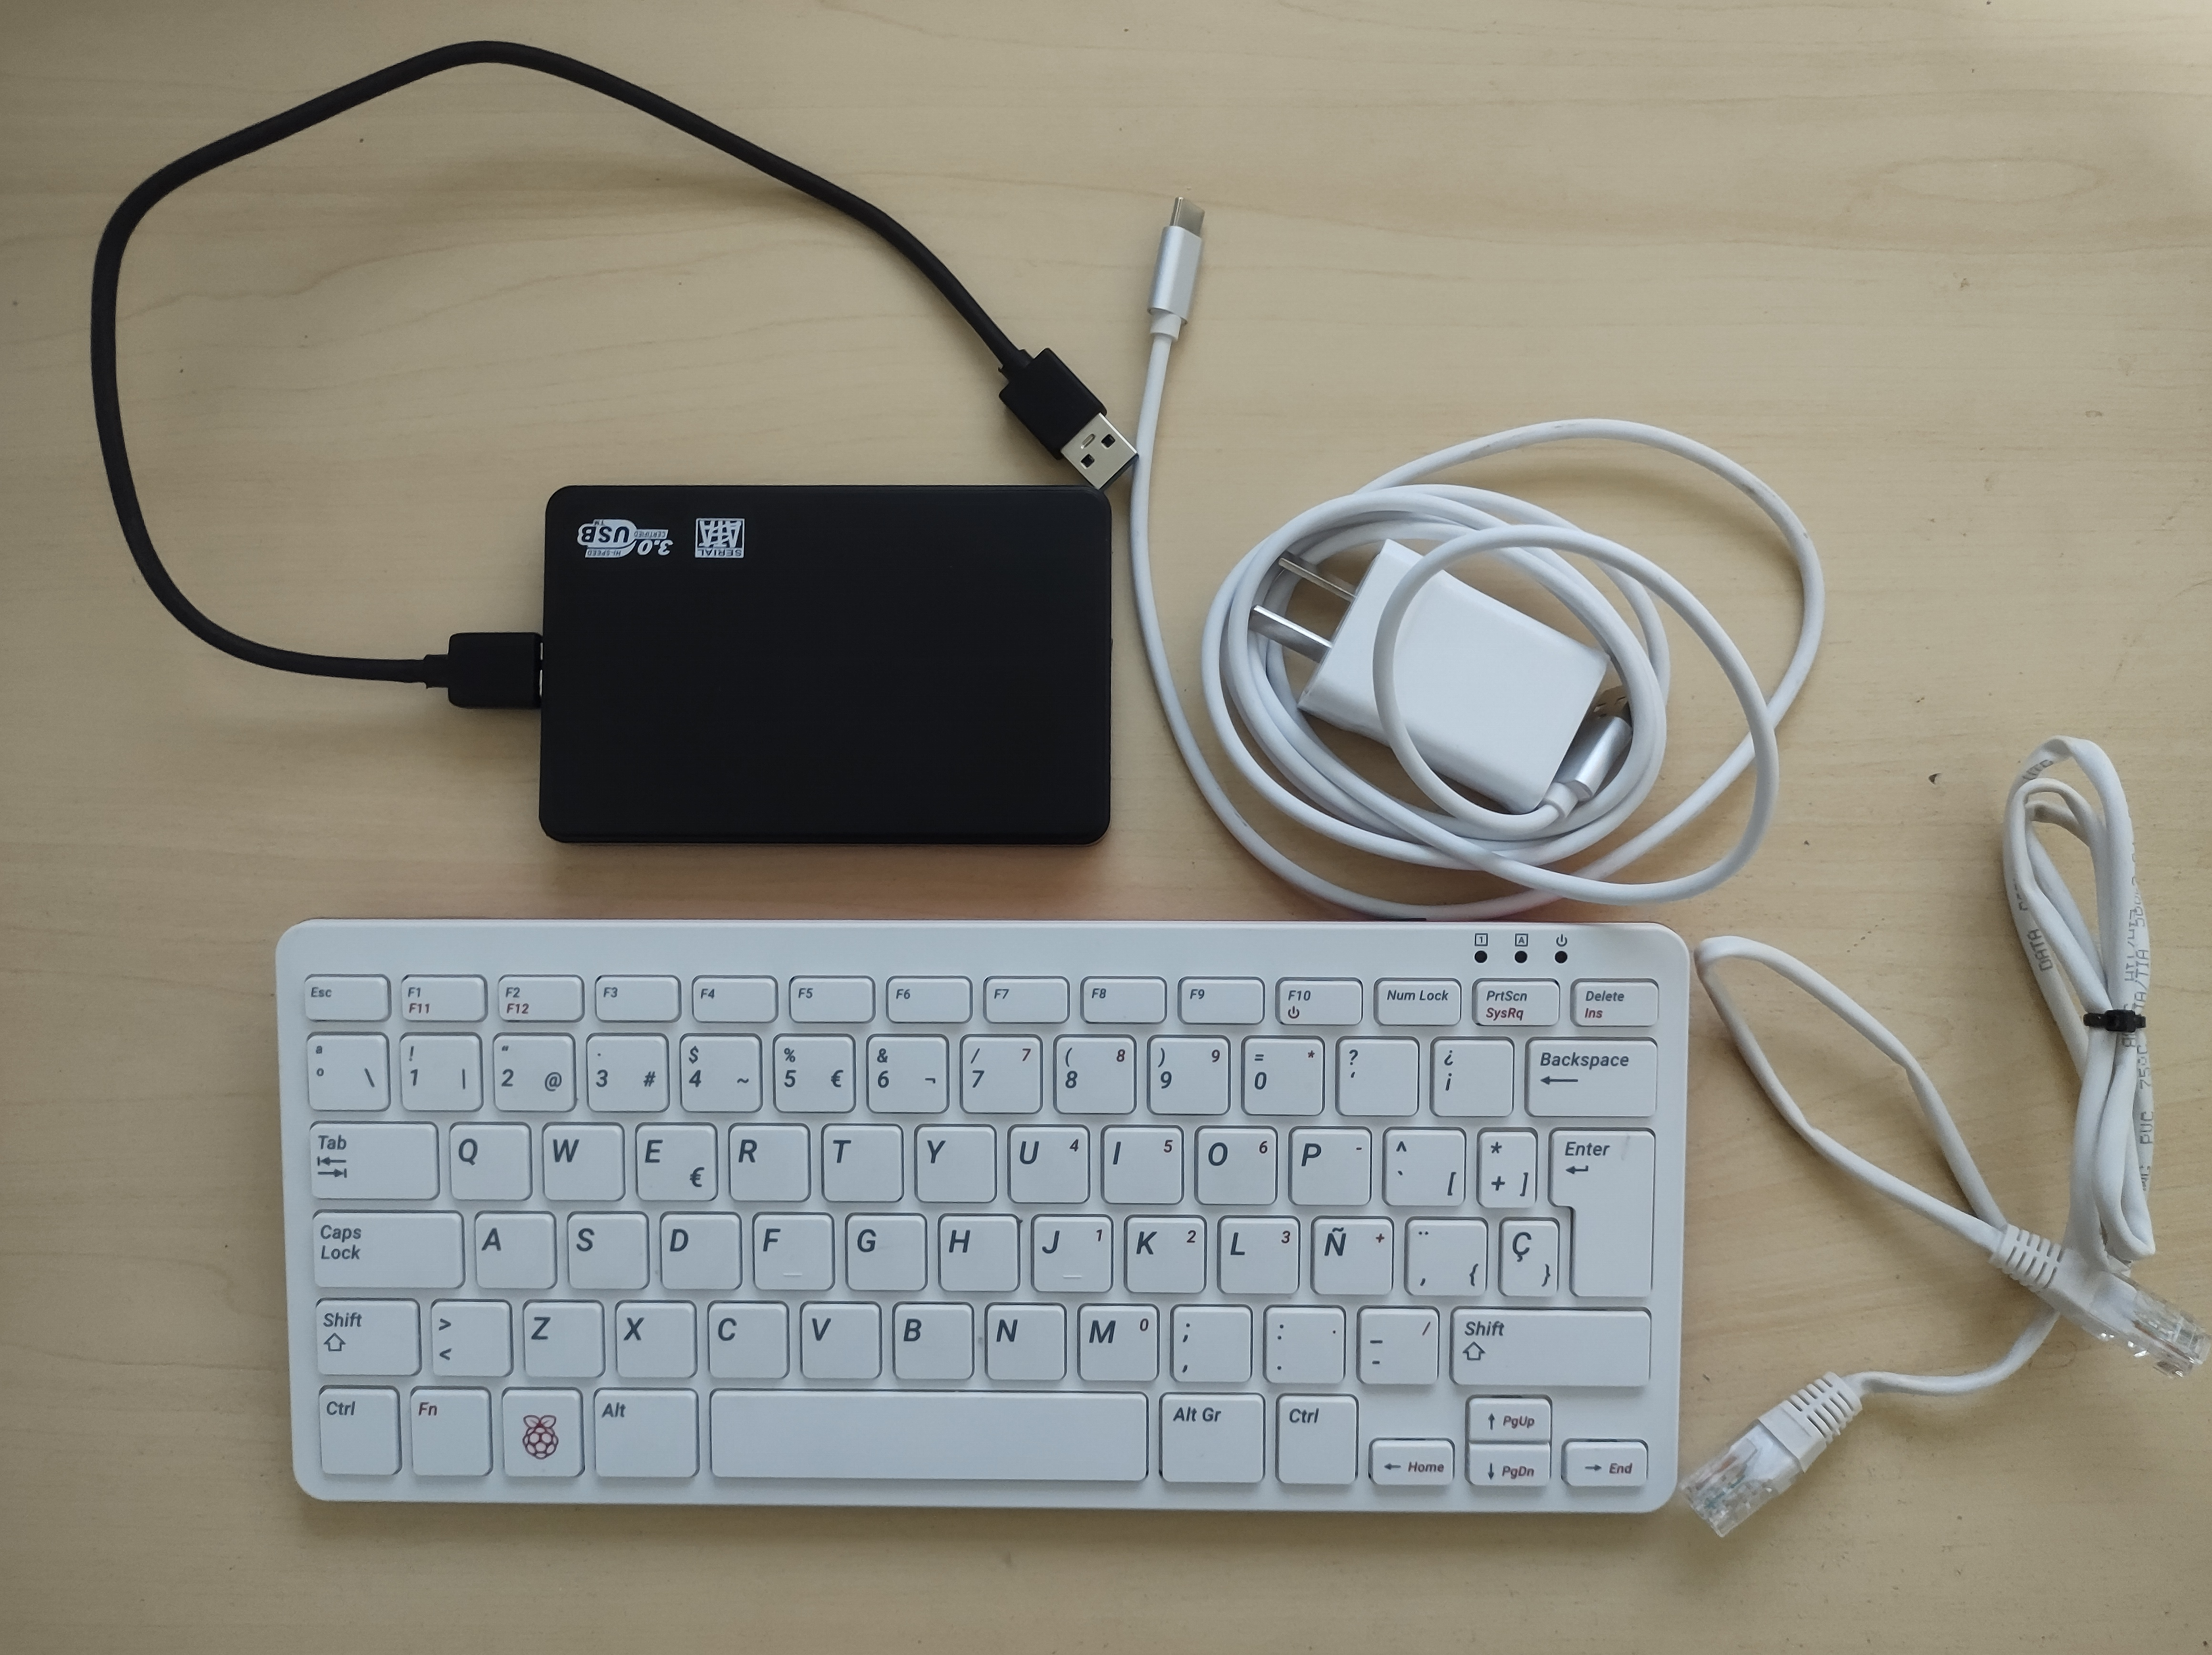
\includegraphics[scale=0.25]{Figura 33 - Servidor.jpg}
\caption[Componentes del servidor]{Componentes del servidor.}
\label{fig:33}
\end{figure}

Puede observarse la Raspberry Pi400, la fuente de 5 VCC 3A con su cable, un disco rígido externo SSD de 120 GB y un cable Ethernet para la conexión a la red.

\section{Metodología empleada}

El hardware se testeó de forma funcional. En cuanto al software se utilizaron distintas metodologías para la depuración de forma manual de los embebidos, el frontend y el backend. A continuación, se describen cada una de ellas.

\subsection{Pruebas del frontend}

Para el frontend se utilizaron pruebas funcionales manuales con el sistema funcionando. El desarrollo fue progresivo y se llevó a cabo en paralelo. Se creó una aplicación básica y, posteriormente, se fueron agregando nuevas funcionalidades. A medida que el sistema fue creciendo, se fueron agregando más componentes hasta tener la versión actual.

En lo que respecta a las pruebas, se empleó la salida de la consola del navegador a medida que se implementaban nuevas funciones y páginas. Esto permitió exhibir en tiempo real el funcionamiento del sistema en cada página y con cada función agregada. En el código \ref{lst:console front} se muestra a modo de ejemplo parte del desarrollo de la página para la visualización de un mensaje por consola de la configuración de un dispositivo.

\begin{lstlisting}[caption={Muestra por consola de los datos recibidos.}, label={lst:console front}]
ngOnInit() {
    const deviceId = this.activatedRoute.snapshot.paramMap.get('id') as string;
    this.dispositivoId = deviceId, 10;
    this.subscription = this.dispositivoService.getDeviceById(this.dispositivoId).
   		subscribe((data) => {
      console.log(data);
      this.device = data[0];
      this.tipo = data[0].tipo;
      this.ubicacion = data[0].ubicacion;
    });
    this.leerdatos();
  }
\end{lstlisting}

Allí se puede ver la función \textit{console.log} mostrando los datos por consola. En la figura \ref{fig:34} se puede ver la pantalla de configuración del dispositivo y el mensaje por consola con los datos recibidos.

\newpage
\begin{figure}[h]
\centering
\includegraphics[scale=0.37]{Figura 34 - Consola front.png}
\caption[Pantalla de aplicación y consola del frontend]{Pantalla de aplicación y consola.}
\label{fig:34}
\end{figure}

Este mecanismo se utilizó en todas las páginas de la aplicación web y gracias a esto se consiguieron los resultados esperados de funcionalidad y depuración de errores.

\subsection{Pruebas del backend}

Para el backend se utilizó un mecanismo similar de pruebas funcionales que para el frontend.

El desarrollo siguió un enfoque progresivo lo que significa que a medida que se fueron incorporando funciones o endpoints nuevos, se fueron colocando muestras por consola para poder observar si los datos y las consultas estaban siendo resueltos de forma correcta. En el código \ref{lst:console back} se muestra como ejemplo el \textit{router} para borrar la tabla de mediciones de un dispositivo y el mensaje por consola de éxito y el ID del dispositivo.

\begin{lstlisting}[caption={Muestra por consola de los datos consultados.}, label={lst:console back}]
borrarTablaRouter.delete('/:id', async function (req, res, next) {
  const id = req.params.id;
  let connection;
  try {
      connection = await pool.getConnection();
      await connection.beginTransaction();
      const deleteMedicionesQuery = 'DELETE FROM Mediciones WHERE dispositivoId = ?';
      await connection.query(deleteMedicionesQuery, id);
      await connection.commit();
      connection.release();
      res.send({ message: 'Mediciones eliminadas exitosamente' }).status(200);
      console.log('Solicitud de eliminacion recibida para dispositivoId:', id);
      } catch (err) {
          if (connection) {
              await connection.rollback();
              connection.release();
          }
          res.send(err).status(400);
          console.log('Error al eliminar mediciones:', err);
      }
  });
\end{lstlisting}

En la figura \ref{fig:35} se puede ver la consola con el mensaje de éxito y el ID del dispositivo cuya tabla de mediciones fue eliminada.

\begin{figure}[h]
\centering
\includegraphics[scale=0.65]{Figura 35 - Consola back.png}
\caption[Mensaje por consola del servidor en el backend]{Mensaje por consola del servidor.}
\label{fig:35}
\end{figure}

Además de estas pruebas, se incorporó el uso de la aplicación \textit{MQTTX} para testear la comunicación con el \textit{broker} y los dispositivos, especialmente durante la implementación de la seguridad con los certificados SSL. De esta forma, se llevaron a cabo pruebas que abarcaron desde la primera conexión segura hasta la inserción de datos desde un dispositivo simulado, el envío de configuración desde la aplicación a los nodos y el mensaje de solicitud de configuración inicial de un nodo, entre otros.

En la figura \ref{fig:36} puede verse la configuración de \textit{MQTTX} para el envío de datos de una medición simulada en el \textit{topic \textbackslash home\textbackslash temperatura\textbackslash data} para luego verificar la correcta inserción en la base de datos.

\begin{figure}[h]
\centering
\includegraphics[scale=0.5]{Figura 36 - MQTTX.png}
\caption[Pantalla de MQTTX]{Pantalla de MQTTX.}
\label{fig:36}
\end{figure}

\subsection{Pruebas de los nodos}

El hardware se testeó haciendo pruebas de funcionamiento con los materiales mencionados en la sección anterior. Las pruebas consistieron en poner en funcionamiento los nodos durante dos días consecutivos, verificando que el control de temperatura funcionara dentro de los valores configurados y que la luminaria se encendiera y mantuviera los valores de los saltos. También se evaluó el funcionamiento de los horarios de encendido y apagado.

En cuanto al software, las placas ESP32 poseen comunicación serial incorporada por lo que se colocaron funciones de muestra por consola al momento de incorporar funcionalidades nuevas. En el código \ref{lst:dispositivo}, se puede ver un ejemplo de cómo se utilizó la función \textit{ESP\_LOGI} para mostrar por consola el valor de la salida recibido por MQTT.

\lstset{frame=tb,
  language=C++,
  aboveskip=3mm,
  belowskip=3mm,
  captionpos=b,
  showstringspaces=false,
  columns=flexible,
  basicstyle={\small\ttfamily},
  numbers=left,
  numberstyle=\tiny\color{gray},
  keywordstyle=\color{blue},
  commentstyle=\color{dkgreen},
  stringstyle=\color{mauve},
  breaklines=true,
  breakatwhitespace=true,
  tabsize=3,
}

\begin{lstlisting}[caption={Muestra por consola de la terminal ESP-IDF.}, label={lst:dispositivo}]
const cJSON *salida = cJSON_GetObjectItemCaseSensitive(root, "salida");
    if (cJSON_IsNumber(salida) && select) {
        if(salida->valueint==100)
            out_temp=true;
        if(salida->valueint==0)
            out_temp=false;
        ESP_LOGI(TAG, "Received MQTT salida: %d", salida->valueint);
        pant_main();
    }
\end{lstlisting}

En este caso se muestra por consola el mensaje de recepción del valor de salida y su valor correspondiente.

\section{Resultados finales}

Para la prueba final, se ensamblaron los 2 nodos, y se conectó un calefactor eléctrico de 750 W al nodo de temperatura. En el lado del servidor, se ejecutó el \textit{docker-compose} con el sistema completo. Se realizaron ajustes tanto desde la aplicación web como de cada uno de los nodos.

En la figura \ref{fig:37}, se puede observar el nodo de iluminación funcionando encendido, y en la pantalla se muestra el valor de la salida.

\begin{figure}[h]
\centering
\includegraphics[scale=0.06]{Figura 37 - Dimmer funcionando.jpg}
\caption[Dimmer en modo automático funcionando]{Dimmer en modo automático funcionando.}
\label{fig:37}
\end{figure}

En la figura \ref{fig:38}, se puede observar la pantalla de configuración de modo automático.

\begin{figure}[h]
\centering
\includegraphics[angle=270, scale=0.47]{Figura 38 - Pantalla dimmer funcionando.jpg}
\caption[Pantalla de configuración del dimmer en modo automático]{Pantalla de configuración del dimmer en modo automático.}
\label{fig:38}
\end{figure}

En la figura \ref{fig:39} puede observarse la página de configuración del nodo dimmer. Puede observarse que los datos ingresados corresponden con los datos guardados en el nodo, y que este último está funcionando según lo esperado.

\begin{figure}[h]
\centering
\includegraphics[scale=0.45]{Figura 39 - Config.png}
\caption[Pantalla de configuración de dimmer]{Pantalla de configuración de dimmer.}
\label{fig:39}
\end{figure}

Se ha verificado la capacidad de agregar y modificar los datos de los dispositivos desde la página correspondiente, contrastando los datos visualizados en la pantalla de \textit{phpMyAdmin}. Durante una prueba que se realizó, se cargó un dispositivo nuevo y se corroboró tanto desde la aplicación del sistema como desde la página de administración de la base de datos. En la figura \ref{fig:40} puede verse cómo se agregó un dispositivo nuevo desde la página en la parte superior y cómo se ve reflejado en la base de datos en la inferior.

\newpage
\begin{figure}[h]
\centering
\includegraphics[scale=0.33]{Figura 40 - Agregar dispositivo.png}
\caption[Valores de dispositivo nuevo al agregar dispositivo]{Valores de dispositivo nuevo.}
\label{fig:40}
\end{figure}

Aquí se observa que los datos cargados coinciden con los almacenados. La diferencia radica en que no se registró la MAC del dispositivo ya que al momento de obtener la imagen el dispositivo no había emitido datos al servidor.

Algo similar a la prueba de los dispositivos se hizo con los usuarios. El sistema por default tiene los valores \textit{user1}, \textit{user2} y \textit{user3} y contraseña \textit{user}. Esto se logró creando estos usuarios con sus datos en el archivo de creación de la base de datos \textit{domotica.sql}. En la figura \ref{fig:41} se muestran los valores ingresados en la página de configuración en la parte superior y los que están almacenados en la base de datos en la inferior. Como se puede observar en la imagen, los valores cargados desde la página coinciden con los almacenados en la base de datos.

\begin{figure}[h]
\centering
\includegraphics[scale=0.34]{Figura 41 - Modificar usuario.png}
\caption[Valores de usuario modificados]{Valores de usuario modificados.}
\label{fig:41}
\end{figure}

Por último, se hizo la corroboración de la activación de la alarma y el envío del mail. En la figura \ref{fig:42} puede observarse la configuración del dispositivo en la parte superior y el mail recibido en la parte inferior.

\begin{figure}[h]
\centering
\includegraphics[scale=0.35]{Figura 42 - Alarma.png}
\caption[Envío de alarma de medición]{Envío de alarma de medición.}
\label{fig:42}
\end{figure}

De esta forma se hicieron las pruebas más importantes de funcionalidades del sistema. Al dar resultados de funcionamiento satisfactorios, se concluye que la aplicación funciona de manera correcta.

\section{Comparación con el estado del arte}

En la tabla \ref{tab:estadoarte} se encuentra la comparación entre las soluciones de hogares inteligentes existentes en el mercado nacional, Domotic y Reactor, y el trabajo realizado. 

\newpage
\begin{table}[h]
\centering
\caption[Comparativa entre las distintas opciones - Estado del arte]{Comparativa entre las distintas opciones.}
\begin{tabular}{l c c c}
\toprule
\textbf{Funcionalidad} & \textbf{Domotic} & \textbf{Reactor} & \textbf{Trabajo final}\\
\midrule
Posee unidad central			& Sí		& No		& Sí\\
Capacidad de diseño de		&		&		&\\
dispositivos nuevos			& Sí		& Sí		& Sí\\
Almacenamiento de mediciones	& No		& Sí		& Sí\\
Programación de reacciones	& Sí		& Sí		& Sí\\
Aplicación en ambientes		&		&		&\\
profesionales y oficinas		& No		& Sí		& Sí\\
Avisos por mail				& No		& Sí		& Sí\\
Aplicación móvil				& Sí		& Sí		& No\\
Conexión	 desde el exterior	& Sí		& Sí		& No\\
\bottomrule
\hline
\end{tabular}
\label{tab:estadoarte}
\end{table}

Como se puede observar de la tabla comparativa, el trabajo está a la par de otras soluciones similares. Entre sus puntos positivos, el sistema desarrollado posee una unidad central, en este caso, el servidor, que puede aceptar diseños nuevos de dispositivos, proporciona notificaciones en caso de eventos y almacena valores de mediciones que sean útiles.

En cuanto a los aspectos a mejorar se describirán en el capítulo 5 en la sección de trabajo futuro. 
\chapter{Conclusiones}

\label{Chapter5}



\section{Resultados obtenidos}


\section{Trabajo futuro}

 

%----------------------------------------------------------------------------------------
%	CONTENIDO DE LA MEMORIA  - APÉNDICES
%----------------------------------------------------------------------------------------

\appendix % indicativo para indicarle a LaTeX los siguientes "capítulos" son apéndices

% Incluir los apéndices de la memoria como archivos separadas desde la carpeta Appendices
% Descomentar las líneas a medida que se escriben los apéndices

%% Appendix A

\chapter{Ejemplo de creación de menú en ESP32} % Main appendix title

En este anexo se describe un ejemplo de manejo del menú principal en los nodos.

\label{AppendixA} % For referencing this appendix elsewhere, use \ref{AppendixA}

\begin{lstlisting}[caption={Código del menú principal.}, label={lst:Ejemplo menu}]
void menu1 (void)
{
	ssd1306_clear_screen(&devd, false);
	pos_menu=1;
	while(level==1){
		if(inc_enc){
			pos_menu++;
			inc_enc=false;
			if (pos_menu>6)
				pos_menu=1;
		}	
		if (dec_enc){
			pos_menu--;
			dec_enc=false;
			if (pos_menu<1)
				pos_menu=6;
		}
		if(pos_menu==1){
			ssd1306_display_text(&devd, 0, "Estado          ", 16, true);
			ssd1306_display_text(&devd, 1, "Info conexion   ", 16, false);
			ssd1306_display_text(&devd, 2, "Modo            ", 16, false);
			ssd1306_display_text(&devd, 3, "Conf modo auto  ", 16, false);
			ssd1306_display_text(&devd, 4, "Actualizar hora ", 16, false);
			ssd1306_display_text(&devd, 5, "Pant. principal ", 16, false);
			if(btn_enc){
				btn_enc=false;
				level=10;
			}
		}
		if(pos_menu==2){
			ssd1306_display_text(&devd, 0, "Estado          ", 16, false);
			ssd1306_display_text(&devd, 1, "Info conexion   ", 16, true);
			ssd1306_display_text(&devd, 2, "Modo            ", 16, false);
			ssd1306_display_text(&devd, 3, "Conf modo auto  ", 16, false);
			ssd1306_display_text(&devd, 4, "Actualizar hora ", 16, false);
			ssd1306_display_text(&devd, 5, "Pant. principal ", 16, false);
			if(btn_enc){
				btn_enc=false;
				level=11;
			}
		}
		if(pos_menu==3){
			ssd1306_display_text(&devd, 0, "Estado          ", 16, false);
			ssd1306_display_text(&devd, 1, "Info conexion   ", 16, false);
			ssd1306_display_text(&devd, 2, "Modo            ", 16, true);
			ssd1306_display_text(&devd, 3, "Conf modo auto  ", 16, false);
			ssd1306_display_text(&devd, 4, "Actualizar hora ", 16, false);
			ssd1306_display_text(&devd, 5, "Pant. principal ", 16, false);	
			if(btn_enc){
				btn_enc=false;
				level=2;
			}
		}
		if(pos_menu==4){
			ssd1306_display_text(&devd, 0, "Estado          ", 16, false);
			ssd1306_display_text(&devd, 1, "Info conexion   ", 16, false);
			ssd1306_display_text(&devd, 2, "Modo            ", 16, false);
			ssd1306_display_text(&devd, 3, "Conf modo auto  ", 16, true);
			ssd1306_display_text(&devd, 4, "Actualizar hora ", 16, false);
			ssd1306_display_text(&devd, 5, "Pant. principal ", 16, false);	
			if(btn_enc){
				btn_enc=false;
				level=3;
			}
		}
		if(pos_menu==5){
			ssd1306_display_text(&devd, 0, "Estado          ", 16, false);
			ssd1306_display_text(&devd, 1, "Info conexion   ", 16, false);
			ssd1306_display_text(&devd, 2, "Modo            ", 16, false);
			ssd1306_display_text(&devd, 3, "Conf modo auto  ", 16, false);
			ssd1306_display_text(&devd, 4, "Actualizar hora ", 16, true);
			ssd1306_display_text(&devd, 5, "Pant. principal ", 16, false);
			if(btn_enc){
				btn_enc=false;
				ssd1306_display_text(&devd, 6, "Obteniendo la", 13, false);
    			ssd1306_display_text(&devd, 7, "hora...", 7, false);
				obtain_time();
				ssd1306_display_text(&devd, 7, "hora... OK", 10, false);
				vTaskDelay(pdMS_TO_TICKS(1000));
				ssd1306_display_text(&devd, 6, "               ", 15, false);
				ssd1306_display_text(&devd, 7, "               ", 15, false);
			}
		}
		if(pos_menu==6){
			ssd1306_display_text(&devd, 0, "Estado          ", 16, false);
			ssd1306_display_text(&devd, 1, "Info conexion   ", 16, false);
			ssd1306_display_text(&devd, 2, "Modo            ", 16, false);
			ssd1306_display_text(&devd, 3, "Conf modo auto  ", 16, false);
			ssd1306_display_text(&devd, 4, "Actualizar hora ", 16, false);
			ssd1306_display_text(&devd, 5, "Pant. principal ", 16, true);
			if (btn_enc){
				btn_enc=false;
				level=0;	
			}
		}
	}
	if(level==10){
			if (net_con)
				pant_conok();
			if (!net_con)
				pant_nocon();
	}
	if(level==11){
		pant_est();
	}
	if(level==2){
		menu2();
	}
	if(level==3){
		menu3();
	}
	if(level==0){
		pant_main();
	}
}
\end{lstlisting}
%\include{Appendices/AppendixB}
%\include{Appendices/AppendixC}

%----------------------------------------------------------------------------------------
%	BIBLIOGRAPHY
%----------------------------------------------------------------------------------------

\Urlmuskip=0mu plus 1mu\relax
\raggedright
\printbibliography[heading=bibintoc]

%----------------------------------------------------------------------------------------

\end{document}  
